% Niveau :      PC
% Discipline :  Mécaflu
%Mots clés :    Tension superficielle

\begin{exercise}{Ascension capillaire}{2}{Spé}
{Statique des fluides, Tension superficielle, Capillarité}{bermu}

\begin{questions}
    \questioncours Rappeler ce que sont les effets de tension de surface et les modéliser rapidement. On définira le coefficient de tension de surface $\gamma$.
\begin{EnvUplevel}
\paragraph{Rappel :} loi de Laplace \\
\`A l'interface entre deux fluides $a$ et $b$ non miscibles, la tension de surface (dont le coefficient est $\gamma_{ab}$) créée une surpression telle que
$$P_b - P_a = \dfrac{2\gamma_{ab}}{R_c},$$
$R_c$ étant le rayon de courbure de l'interface.

\begin{multicols}{2}
\begin{figure}[H]
    \centering
    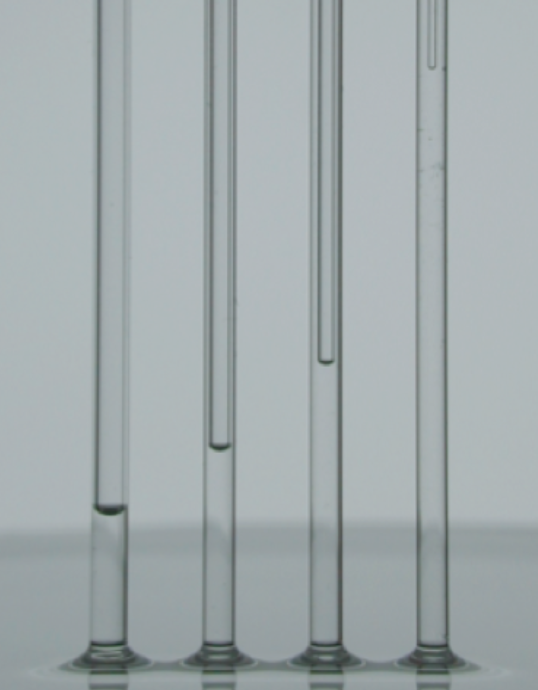
\includegraphics[width=\linewidth]{mecaflu/jurin1.png}
    \vspace{-1em}
    \caption{Ascension capillaire dans des tubes de différentes tailles.}\label{fig:jur1}
\end{figure}
\begin{figure}[H]
    \centering
    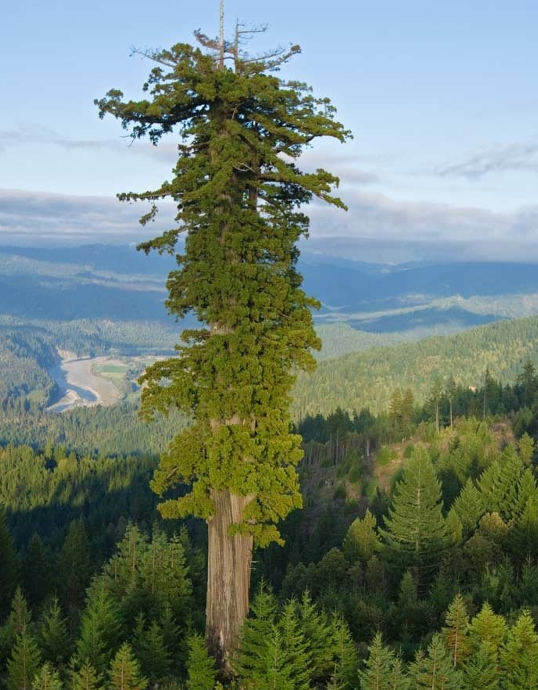
\includegraphics[width=\linewidth]{mecaflu/jurin2.png}
    \vspace{-1em}
    \caption{\emph{Hypérion}, l'arbre le plus haut du monde.}\label{fig:jur2}
\end{figure}
\end{multicols}

\end{EnvUplevel}
    \question \`A l'aide de la loi de Laplace, expliquer la figure \ref{fig:jur1} ci-dessus et estimer la tension superficielle eau--air. \\
    On appellera $\theta$ l'angle de contact entre le ménisque (que l'on supposera être une calote sphérique) et le tube.
\uplevel{L'arbre le plus haut du monde, un séquoia nommé \emph{Hypérion}  et situé dans le parc national de \emph{Redwood} en Californie (fig.~\ref{fig:jur2}), mesure 115m.}
    \question Estimer jusqu'à quelle hauteur limite la sève peut monter dans l'arbre par capillarité. \\
    Quelle peut être une autre raison de l'ascension de la sève dans les arbres ?
\end{questions}
\end{exercise}